% Drawing 69/04-5 -- folder 69, batch 04, archive page 78 (PDF page 79).
% Transcription: en haut à gauche, une étoile de dix rayons issus d'un point $s$, les extrémités marquées $\circ$, $\bullet$, $\times$, $*$, $\alpha_1$, $\alpha'_1$, $\alpha_2$, $\alpha'_2$ ; un petit parallélogramme fléché ; un carré aux sommets $\bullet$, $\times$, $\circ$ ; un tableau $2\times2$ de lignes $\alpha_2$, $\alpha'_2$ et colonnes $\alpha_1$, $\alpha'_1$, garni de $\circ$, $*$, $\times$, $\bullet$ ; un cube aux sommets marqués $0$, $e_1$, $e_2$, $e_3$, $e_1+e_2$, $e_1+e_3$, $e_2+e_3$, $e_1+e_2+e_3$ ; un hexagone entouré de trois arcs joignant ses sommets $\alpha_1$, $\alpha'_1$, $\alpha_2$, $\alpha'_2$ à un point $s$ ; deux boîtes en perspective ; une figure d'éventails autour de sommets $1$, $1''$, $2'$, $\alpha'_1$ ; en bas, trois graphes à sommets $u$, $v$, $w$, $\sigma_4$, $\alpha'_3$, $\alpha_4$, $\beta_3$, $\beta_4$, un éventail de triangles, un octaèdre marqué $w$ ; enfin deux lignes $\alpha'_3,\alpha'_4$ / $\beta'_2,\beta'_1,\beta'_3,\beta'_4$ / $\beta_1,\beta_2,\beta_3,\beta'_4$ et, en bas à droite, « $2\cdot6\cdot8$ ».
% Kind: page of sketches (star, table, cube, hexagon, fans, graphs, octahedron). Method 2 (schematic redraw from the facsimile). Status: partial.
% Notes: Whole page. Drawn schematically at their places: the ten-ray star from s with the end marks, the small arrowed parallelogram, the square with marked corners, the 2x2 table, the cube with 0, e_i, e_i+e_j, the hexagon with three arcs to s, two boxes, the fan figure around 1, 1'', 2', the three graphs on u, v, w, the fan of triangles, the octahedron, the two lines of letters and 2.6.8. Formulas and the I~ diagram are not drawn. Strokes approximate (the fan figure is heavily inked); end marks and small labels after the transcription where illegible.
% Coordinates: 1 unit = 1 mm = 1/100 of the crop width (bbox in page fractions: [0.06, 0.05, 0.95, 0.85]).
% Redrawn by Claude (claude-opus-5-5), issue #73, 2026-11-07; not checked by a human; not compiled (no TeX in the session).
% Rights: reproduces part of the work -- behind RENDER_TRANSCRIPTS, never published by itself.
\documentclass[tikz,border=3pt]{standalone}
\usepackage{amsmath,amssymb}
\usetikzlibrary{patterns,arrows.meta}
\tikzset{pencil/.style={black!45}, struck/.style={black!35}, mark/.style={circle,draw,inner sep=1.3pt}, pt/.style={circle,fill,inner sep=0.9pt}, opt/.style={circle,draw,fill=white,inner sep=1.1pt}}
\begin{document}
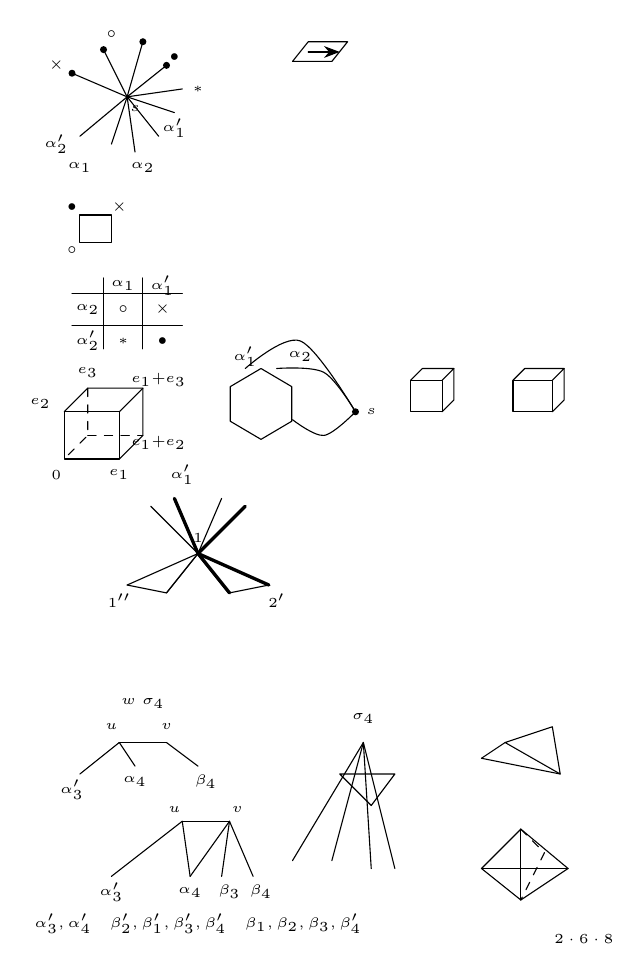
\begin{tikzpicture}[x=1mm,y=1mm,line cap=round,line join=round,font=\scriptsize]
\draw (21,-18) -- (14,-15);
\draw (21,-18) -- (18,-12);
\draw (21,-18) -- (23,-11);
\draw (21,-18) -- (26,-14);
\draw (21,-18) -- (28,-17);
\draw (21,-18) -- (27,-20);
\draw (21,-18) -- (25,-23);
\draw (21,-18) -- (22,-25);
\draw (21,-18) -- (19,-24);
\draw (21,-18) -- (15,-23);
\node[pt] at (14,-15) {};
\node[pt] at (18,-12) {};
\node[pt] at (23,-11) {};
\node[pt] at (26,-14) {};
\node[inner sep=1pt] at (22,-19.5) {\tiny $s$};
\node[inner sep=1pt] at (12,-14) {\tiny $\times$};
\node[inner sep=1pt] at (19,-10) {\tiny $\circ$};
\node[inner sep=1pt] at (27,-13) {\tiny $\bullet$};
\node[inner sep=1pt] at (30,-17) {\tiny $*$};
\node[inner sep=1pt] at (15,-27) {\tiny $\alpha_1$};
\node[inner sep=1pt] at (27,-22) {\tiny $\alpha'_1$};
\node[inner sep=1pt] at (23,-27) {\tiny $\alpha_2$};
\node[inner sep=1pt] at (12,-24) {\tiny $\alpha'_2$};
\draw (42,-13.5) -- (44,-11) -- (49,-11) -- (47,-13.5) -- cycle;
\draw[-{Stealth[length=2mm]}] (44,-12.3) -- (48,-12.3);
\draw (15,-33) -- (19,-33) -- (19,-36.5) -- (15,-36.5) -- cycle;
\node[inner sep=1pt] at (14,-32) {\tiny $\bullet$};
\node[inner sep=1pt] at (20,-32) {\tiny $\times$};
\node[inner sep=1pt] at (14,-37.5) {\tiny $\circ$};
\draw (14,-43) -- (28,-43);
\draw (14,-47) -- (28,-47);
\draw (18,-41) -- (18,-50);
\draw (23,-41) -- (23,-50);
\node[inner sep=1pt] at (20.5,-42) {\tiny $\alpha_1$};
\node[inner sep=1pt] at (25.5,-42) {\tiny $\alpha'_1$};
\node[inner sep=1pt] at (16,-45) {\tiny $\alpha_2$};
\node[inner sep=1pt] at (16,-49) {\tiny $\alpha'_2$};
\node[inner sep=1pt] at (20.5,-45) {\tiny $\circ$};
\node[inner sep=1pt] at (25.5,-45) {\tiny $\times$};
\node[inner sep=1pt] at (20.5,-49) {\tiny $*$};
\node[inner sep=1pt] at (25.5,-49) {\tiny $\bullet$};
\draw (13,-58) -- (20,-58) -- (20,-64) -- (13,-64) -- cycle;
\draw (16,-55) -- (23,-55) -- (23,-61) -- (20,-64);
\draw (13,-58) -- (16,-55);
\draw (20,-58) -- (23,-55);
\draw[dashed] (16,-55) -- (16,-61) -- (13,-64);
\draw[dashed] (16,-61) -- (23,-61);
\node[inner sep=1pt] at (12,-66) {\tiny $0$};
\node[inner sep=1pt] at (20,-66) {\tiny $e_1$};
\node[inner sep=1pt] at (10,-57) {\tiny $e_2$};
\node[inner sep=1pt] at (16,-53) {\tiny $e_3$};
\node[inner sep=1pt] at (25,-54) {\tiny $e_1{+}e_3$};
\node[inner sep=1pt] at (25,-62) {\tiny $e_1{+}e_2$};
\draw (38,-52.5) -- (34.1,-54.8) -- (34.1,-59.2) -- (38,-61.5) -- (41.9,-59.2) -- (41.9,-54.8) -- cycle;
\draw plot[smooth, tension=0.55] coordinates {(36,-52.5) (43,-49) (50,-58)};
\draw plot[smooth, tension=0.55] coordinates {(40,-52.5) (46,-53) (50,-58)};
\draw plot[smooth, tension=0.55] coordinates {(42,-59) (46,-61) (50,-58)};
\node[pt] at (50,-58) {};
\node[inner sep=1pt] at (52,-58) {\tiny $s$};
\node[inner sep=1pt] at (36,-51) {\tiny $\alpha'_1$};
\node[inner sep=1pt] at (43,-51) {\tiny $\alpha_2$};
\draw (57,-54) -- (61,-54) -- (61,-58) -- (57,-58) -- cycle;
\draw (57,-54) -- (58.5,-52.5) -- (62.5,-52.5) -- (61,-54);
\draw (62.5,-52.5) -- (62.5,-56.5) -- (61,-58);
\draw (70,-54) -- (75,-54) -- (75,-58) -- (70,-58) -- cycle;
\draw (70,-54) -- (71.5,-52.5) -- (76.5,-52.5) -- (75,-54);
\draw (76.5,-52.5) -- (76.5,-56.5) -- (75,-58);
\draw (30,-76) -- (24,-70);
\draw[very thick] (30,-76) -- (27,-69);
\draw (30,-76) -- (33,-69);
\draw[very thick] (30,-76) -- (36,-70);
\draw (30,-76) -- (21,-80);
\draw[very thick] (30,-76) -- (39,-80);
\draw (30,-76) -- (26,-81);
\draw[very thick] (30,-76) -- (34,-81);
\draw (21,-80) -- (26,-81) -- (30,-76);
\draw (34,-81) -- (39,-80);
\node[inner sep=1pt] at (30,-74) {\tiny $1$};
\node[inner sep=1pt] at (20,-82) {\tiny $1''$};
\node[inner sep=1pt] at (40,-82) {\tiny $2'$};
\node[inner sep=1pt] at (28,-66) {\tiny $\alpha'_1$};
\draw (20,-100) -- (26,-100);
\draw (20,-100) -- (15,-104);
\draw (20,-100) -- (22,-103);
\draw (26,-100) -- (30,-103);
\node[inner sep=1pt] at (19,-98) {\tiny $u$};
\node[inner sep=1pt] at (26,-98) {\tiny $v$};
\node[inner sep=1pt] at (23,-95) {\tiny $w\ \sigma_4$};
\node[inner sep=1pt] at (14,-106) {\tiny $\alpha'_3$};
\node[inner sep=1pt] at (22,-105) {\tiny $\alpha_4$};
\node[inner sep=1pt] at (31,-105) {\tiny $\beta_4$};
\draw (28,-110) -- (34,-110);
\draw (28,-110) -- (19,-117);
\draw (28,-110) -- (29,-117);
\draw (34,-110) -- (29,-117);
\draw (34,-110) -- (33,-117);
\draw (34,-110) -- (37,-117);
\node[inner sep=1pt] at (27,-108.5) {\tiny $u$};
\node[inner sep=1pt] at (35,-108.5) {\tiny $v$};
\node[inner sep=1pt] at (19,-119) {\tiny $\alpha'_3$};
\node[inner sep=1pt] at (29,-119) {\tiny $\alpha_4$};
\node[inner sep=1pt] at (34,-119) {\tiny $\beta_3$};
\node[inner sep=1pt] at (38,-119) {\tiny $\beta_4$};
\draw (51,-100) -- (42,-115);
\draw (51,-100) -- (47,-115);
\draw (51,-100) -- (52,-116);
\draw (51,-100) -- (55,-116);
\draw (48,-104) -- (52,-108) -- (55,-104) -- cycle;
\node[inner sep=1pt] at (51,-97) {\tiny $\sigma_4$};
\draw (69,-100) -- (75,-98) -- (76,-104) -- cycle;
\draw (66,-102) -- (69,-100);
\draw (66,-102) -- (76,-104);
\draw (66,-116) -- (71,-111) -- (77,-116) -- (71,-120) -- cycle;
\draw (66,-116) -- (77,-116);
\draw (71,-111) -- (71,-120);
\draw[dashed] (71,-111) -- (74,-114) -- (71,-120);
\node[inner sep=1pt] at (30,-123) {\tiny $\alpha'_3,\alpha'_4 \quad \beta'_2,\beta'_1,\beta'_3,\beta'_4 \quad \beta_1,\beta_2,\beta_3,\beta'_4$};
\node[inner sep=1pt] at (79,-125) {\tiny $2\cdot 6\cdot 8$};
\end{tikzpicture}
\end{document}
